\newpage
\section{Auswertung}

In diesem Abschnitt wird der Versuc hausgewertet.

\subsection{gedämpften Schwingung}
Zunächst wird bei einer gedämpften Schwingung die Zeitabhängigkeit der Amplitude untersucht, um den effektiven Dämpfungswiderstand bestimmen zu können.
Dabei wird zunächst die in der Messung bestimmte Amplitudenspitzen in die \autoref{tab:1} eingetragen.

\begin{table}
    \centering
    \caption{Gemessene Spannungsamplituden in Abhängigkeit von der Zeit}
    \label{tab:1}
    \begin{tabular} {S[table-format=4.1] S[table-format=2.2]}
        \toprule
        {$t \mathbin{/} \si{\micro\second}$} & {$U \mathbin{/} \si{\volt}$}  \\
    \midrule
    0 	    &  -82   \\
    12.5 	&   76   \\
    25.5	&  -64   \\
    40  	&   56   \\
    55	    &  -48   \\
    67.5	&   40   \\	
    80	    &  -36   \\
    93.75	&   32   \\
    107.5	&  -26   \\
    122.5	&   22   \\
    135	    &  -20   \\
    148.75  &	16  \\
    162.5	&  -14  \\
    175	    &   11  \\
    188.75  &	-10 \\
    202.5	&   9 \\
    216.25  &	-8 \\
    \bottomrule
\end{tabular}
\end{table}

\noindent
Es reicht jedoch die Einhüllende zu betrachten. Da die Einhüllende unterhalb der X-Achse und Oberhalb sich um einen Vorzeichen unterscheiden, kann 
zur Modelierung dieser, lediglich der Betrag der gemessen Spannung betrachtet werden. Daraus folgen die Grafiken (\ref{fig:1}), in welcher die Zeit gegen die Spannung und gegen den 
Spannungsbetrag aufgetragen werden.

\newpage
\begin{figure}
    \centering
    \label{fig:1}
    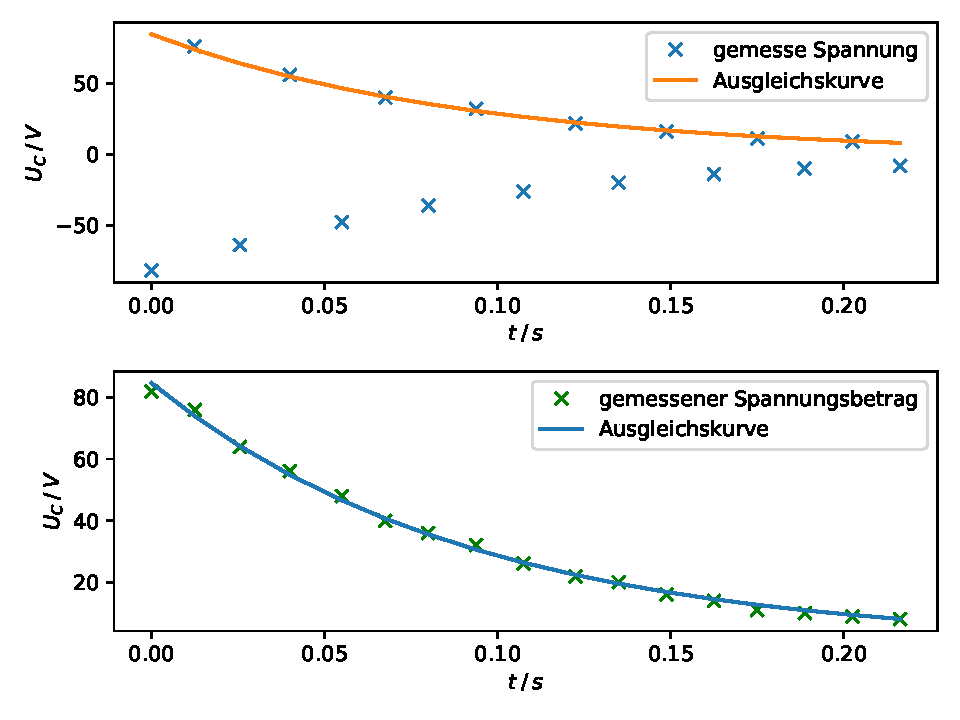
\includegraphics{Daten/a.pdf}
    \caption{Gemessene Spannungsamplituden mit Ausgleichsfunktion}
\end{figure}

Um die Einhüllende zu modelieren, kann diese in der Form
\begin{equation}
    U = a \symup{e}^{b*t}
\end{equation}

\noindent
angenommen werden. Aus der Theorie gilt mit der \autoref{eqn:einh} der Zusammenhang $a = U_0$ und $b = -2 \pi \mu$. Daraus folgt %U_0 e^-2*pi*my*t


\begin{align*}
    a &= 84.684 \pm 0.831 \Leftrightarrow U_0 = 84.684 \pm 0.831 \si{\volt} \\
    b &= -10.8530 \pm 0.17499 \Leftrightarrow \mu = 1.727 \pm 0.027 \si{\per\second} \, .\\
\end{align*}

Mit der Beziehung 
\begin{equation}
    R_\text{eff} = 4\pi\mu L 
\end{equation}
lässt sich der Dämpfungswiderstand R, mit $L = 3.5 \pm 0.01 \si{\milli\henry}$ zu
\begin{equation*}
    R_\text{eff} = 0.0760 \pm 0.0012 \si{\ohm}
\end{equation*}
bestimmen. Damit ist die Abweichung des im verbauten Widerstands $R = 30,3 \pm 0,1 \si{\ohm}$ $99.749 \pm 00.004 \si{\percent}$.

\noindent
Die Abklingdauer kann mithilfe der Formel 
\begin{equation*}
    T_\text{ex} = \frac{1}{2\pi\mu} 
\end{equation*}
berechnet werden zu
\begin{align*}
    T_\text{ex} = 0.011808 \pm 0.007830 \si{\second} \, . \\
\end{align*}



\subsection{aperiodische Grenzfall}
Zusätzlich lässt sich der Dämpfungswiderstand $R_\text(ap)$ experimentell bestimmen zu $R_ap = 12,725 \si{\ohm}$. Der theoretische Wert lässt sich mit der Formel (\ref{eqn:rap}) %R = 2(L/C)^1/2
mit den gegeben Werten
\begin{align*}
   R &= 30,3 \pm 0,1 \si{\ohm}
   L &= 3.5 \pm 0.01 \si{\milli\henry}
   C &= \pm \si{\nano\farad}    
\end{align*}

\noindent
aus dem Aufbau bestimmen. Daraus folgt $$ R_\text(ap) = \si{\ohm} $$ mit einer Abweichung von $ \pm \si{\percent}$.

\subsection{Serienresonanzkreis}
